\documentclass[sigconf,nonacm]{acmart}

% ── Packages ──────────────────────────────────────────────────────────────────
\usepackage{listings}
\usepackage{xcolor}
\usepackage{booktabs}
\usepackage{tikz}
\usepackage{tcolorbox}
\usepackage{multicol}
\usepackage{enumitem}
\usepackage{graphicx}

\tcbuselibrary{skins,breakable}

% ── TODO box ──────────────────────────────────────────────────────────────────
\newtcolorbox{todobox}[1][]{
  colback=yellow!10,
  colframe=orange!80!black,
  fonttitle=\bfseries,
  title={TODO},
  #1
}

% ── Image placeholder box ────────────────────────────────────────────────────
\newtcolorbox{imgplaceholder}[1][]{
  colback=gray!10,
  colframe=gray!60!black,
  fonttitle=\bfseries,
  title={Figure Placeholder},
  #1
}

% ── Code listing style ───────────────────────────────────────────────────────
\definecolor{codebg}{RGB}{248,248,248}
\definecolor{keyword}{RGB}{0,0,180}
\definecolor{string}{RGB}{0,128,0}
\definecolor{comment}{RGB}{128,128,128}
\definecolor{pykey}{RGB}{175,0,219}

\lstdefinelanguage{orca}{
  keywords={model, agent, tool, task, workflow, trigger, schema, input, edge, true, false, null},
  keywordstyle=\color{keyword}\bfseries,
  commentstyle=\color{comment}\itshape,
  stringstyle=\color{string},
  morecomment=[l]{//},
  morecomment=[l]{\#},
  morestring=[b]",
  morestring=[s]{```}{```},
  sensitive=true,
}

\lstdefinestyle{orcaStyle}{
  language=orca,
  backgroundcolor=\color{codebg},
  basicstyle=\ttfamily\scriptsize,
  breaklines=true,
  frame=single,
  framerule=0.4pt,
  rulecolor=\color{gray!50},
  numbers=left,
  numberstyle=\tiny\color{gray},
  tabsize=2,
  captionpos=b,
  aboveskip=6pt,
  belowskip=4pt,
  xleftmargin=1.5em,
  framexleftmargin=1.5em,
  showspaces=false,
  showstringspaces=false,
}

\lstdefinestyle{pythonStyle}{
  language=Python,
  backgroundcolor=\color{codebg},
  basicstyle=\ttfamily\scriptsize,
  breaklines=true,
  frame=single,
  framerule=0.4pt,
  rulecolor=\color{gray!50},
  numbers=left,
  numberstyle=\tiny\color{gray},
  tabsize=2,
  captionpos=b,
  aboveskip=6pt,
  belowskip=4pt,
  xleftmargin=1.5em,
  framexleftmargin=1.5em,
  keywordstyle=\color{pykey}\bfseries,
  stringstyle=\color{string},
  commentstyle=\color{comment}\itshape,
}

\lstset{style=orcaStyle}

% ── Metadata ─────────────────────────────────────────────────────────────────
\title{Compiling Intent: An Agentic Compiler for Multi-Agent System Generation}

\author{Thakee Nathees}
\email{t.abdulmaj@student.curtin.edu.au}
\affiliation{%
  \institution{Curtin University}
  \department{Department of Computing}
  \city{Perth}
  \country{Australia}
}

\begin{document}

\begin{abstract}
The prevailing approach to building multi-agent systems---chaining large
language model (LLM) prompts in sequence---produces systems that are
fragile, non-deterministic, and difficult to debug. When one agent in a
chain produces ambiguous output, subsequent agents fail unpredictably,
causing cascaded errors across the entire pipeline. This paper argues
that the path to robust multi-agent systems lies not in smarter
prompting but in smarter engineering: applying classical compiler design
principles to the orchestration of AI agents. We present a four-phase
architecture---\emph{parsing}, \emph{semantic analysis},
\emph{optimization}, and \emph{code generation}---that transforms
unstructured natural language intent into a deterministic, executable
agent graph. Each phase maps directly to its compiler analogue: prompt
decomposition mirrors lexical analysis, capability validation mirrors
type checking, concurrency detection mirrors optimization passes, and
stateful orchestration mirrors code generation. We further describe an
implementation of this architecture as a self-hosted agentic compiler
written in Orca, a declarative domain-specific language for agent
orchestration, which produces \texttt{.orca} source files that are then
compiled by the Orca compiler into Python/LangGraph code---creating a
two-stage pipeline that isolates LLM non-determinism from deterministic
compilation.
\end{abstract}

\maketitle

% ══════════════════════════════════════════════════════════════════════════════
\section{Introduction}
\label{sec:intro}
% ══════════════════════════════════════════════════════════════════════════════

The current landscape of multi-agent AI systems is dominated by a
pattern that might be called \emph{prompt chaining}: developers connect
large language models in sequence, hoping that autonomous behavior
emerges from interconnected natural language instructions. The typical
architecture is deceptively simple:

\begin{center}
\texttt{User Intent} $\rightarrow$ \texttt{[Agent 1]} $\rightarrow$
\texttt{[Agent 2]} $\rightarrow$ \texttt{[Agent 3]} $\rightarrow$
\texttt{Output}
\end{center}

This approach works adequately for simple workflows---summarizing an
email and creating a calendar invite, for instance. However, it fails
catastrophically for the multi-step, tool-rich problems that distributed
agent systems are meant to solve. Consider a realistic enterprise task:
\emph{``Analyze our last 100 customer churn interviews, find common
technical complaints, cross-reference them with Jira ticket frequency,
and prioritize the top 5 product fixes for the next sprint.''} A
monolithic prompt given to even the most capable model will run out of
context or produce vague generalities. A simple chain will break at the
first ambiguous intermediate output, wasting tokens and causing cascaded
hallucinations.

The fundamental problem is that prompt chaining treats interconnected
black boxes as an engineering methodology. There is no structured
decomposition of the problem, no validation that intermediate outputs
conform to expected schemas, no analysis of which steps can execute
concurrently, and no mechanism to trace failures back to their root
cause.

We observe that this problem has been solved before---in compiler
design. A compiler does not simply concatenate source code
transformations in a linear chain. It \emph{parses} unstructured input
into a structured representation, \emph{validates} that representation
against semantic rules, \emph{optimizes} the resulting graph, and
\emph{generates} executable code for a target environment. Each phase
has a well-defined contract with the next, enabling precise error
reporting, principled optimization, and deterministic output.

This paper presents an architecture for multi-agent systems that applies
these compiler design principles systematically. We make the following
contributions:

\begin{enumerate}[leftmargin=*]
  \item A \textbf{four-phase architecture} for agentic systems that maps
        classical compiler stages---lexical analysis, semantic analysis,
        optimization, and code generation---to agent orchestration,
        replacing ad hoc prompt chains with a principled pipeline.
  \item A \textbf{concrete implementation} of this architecture as a
        self-hosted agentic compiler written in Orca, a declarative DSL
        for agent orchestration, demonstrating that the compiler can
        compile itself.
  \item A \textbf{two-stage compilation pipeline} that isolates LLM
        non-determinism (natural language $\rightarrow$ Orca) from
        deterministic compilation (Orca $\rightarrow$ Python/LangGraph),
        using the Orca compiler's static analysis as a safety net for
        LLM-generated code.
\end{enumerate}

% ══════════════════════════════════════════════════════════════════════════════
\section{Background}
\label{sec:background}
% ══════════════════════════════════════════════════════════════════════════════

\subsection{The Fragility of Prompt Chains}
\label{sec:background:fragility}

The dominant approach to multi-agent systems treats each agent as an
opaque function that consumes and produces natural language. Frameworks
such as LangGraph~\cite{langgraph}, AutoGen~\cite{autogen}, and
CrewAI~\cite{crewai} provide primitives for connecting these functions,
but the developer is responsible for ensuring that outputs conform to
expectations, that failures are handled gracefully, and that the overall
workflow is logically coherent. In practice, this means that a bug in
Agent~A's output---a missing JSON field, an unexpected format, an
ambiguous phrasing---propagates silently through the chain until it
causes a visible failure in Agent~C, far from the root cause.

This fragility stems from the absence of the structural guarantees that
compiler-based systems take for granted: typed interfaces between
components, static validation before execution, and structured error
reporting with source locations.

\subsection{The Orca Language}
\label{sec:background:orca}

Orca is a declarative domain-specific language for AI agent
orchestration, described in a companion paper. It uses an
HCL-inspired~\cite{terraform} block syntax to define models, agents,
tools, tasks, and workflows in a concise notation that compiles to
Python/LangGraph code. The Orca compiler performs static semantic
analysis---reference resolution, type checking, and schema
validation---catching at compile time errors that would otherwise
surface only at runtime. For example:

\begin{lstlisting}[caption={An Orca program defining a two-agent
  research pipeline.},label={fig:orca-example}]
model gpt4 {
  provider    = "openai"
  model_name  = "gpt-4o"
  temperature = 0.2
}

tool web_search {
  name = "web_search"
}

agent researcher {
  model   = gpt4
  tools   = [web_search]
  persona = "You research topics thoroughly."
}

agent writer {
  model   = gpt4
  persona = "You are a technical writer."
}

workflow pipeline {
  flow = researcher -> writer
}
\end{lstlisting}

This program compiles to a LangGraph state graph with two nodes, proper
tool bindings, and source-mapped annotations. The compiler rejects
undefined references (e.g., referencing a model that does not exist),
type mismatches (e.g., assigning a string where a model reference is
expected), and missing required fields---all before any LLM is invoked.

\subsection{Compiler Design Principles}
\label{sec:background:compiler}

A classical compiler transforms source code through a sequence of
well-defined phases, each with a precise contract:

\begin{enumerate}[leftmargin=*]
  \item \textbf{Lexical analysis and parsing}: raw text is decomposed
        into tokens and assembled into an Abstract Syntax Tree (AST), a
        structured, hierarchical representation of the program's intent.
  \item \textbf{Semantic analysis}: the AST is validated against the
        language's type system and scoping rules---variable type
        mismatches, undefined references, and scope violations are
        caught before execution.
  \item \textbf{Optimization}: the validated representation is
        transformed to eliminate dead code, identify parallelism, and
        reduce resource consumption.
  \item \textbf{Code generation}: the optimized representation is
        translated into executable instructions for the target
        environment.
\end{enumerate}

We argue that each of these phases has a direct analogue in multi-agent
system orchestration, and that applying them systematically produces
systems that are more reliable, observable, and efficient than ad hoc
prompt chains.

% ══════════════════════════════════════════════════════════════════════════════
\section{The Compiled Approach}
\label{sec:architecture}
% ══════════════════════════════════════════════════════════════════════════════

Figure~\ref{fig:compiling-intent} contrasts the na\"ive prompt chain
approach with the compiled approach. Rather than passing natural
language between opaque agents, the compiled approach decomposes the
user's intent into a structured, deterministic task graph---an
\emph{Abstract Task Tree} (ATT)---before any worker agent is invoked.

\begin{figure}[t]
\centering
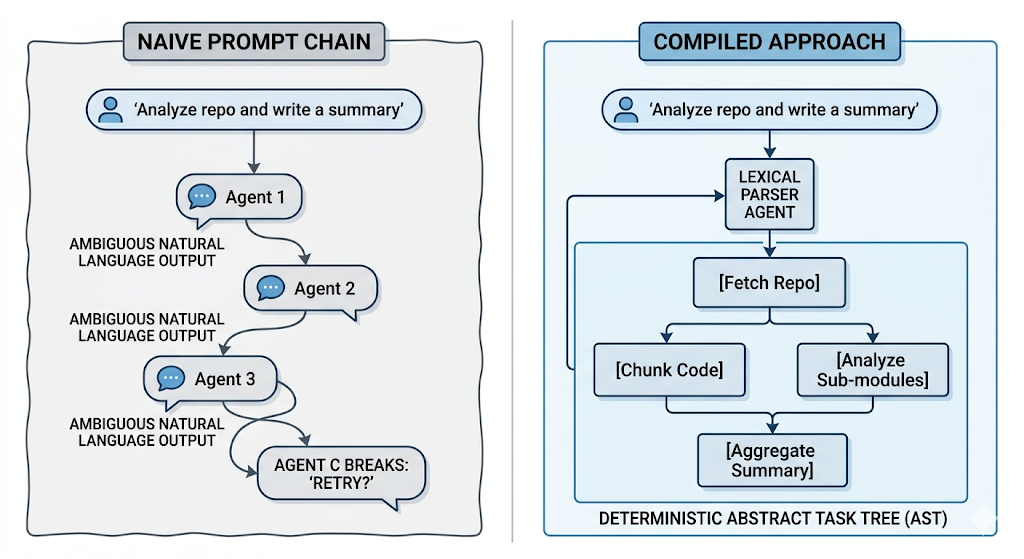
\includegraphics[width=\columnwidth]{figures/compiling-intent.png}
\caption{Na\"ive prompt chaining (left) versus the compiled approach
  (right). The compiled approach decomposes the user's prompt into a
  structured Abstract Task Tree through lexical analysis and semantic
  validation before invoking worker agents.}
\label{fig:compiling-intent}
\end{figure}

The architecture follows a four-phase pipeline, each phase mapping to
its classical compiler analogue:

\begin{center}
\texttt{Natural Language}
$\xrightarrow{\text{Parse}}$ ATT
$\xrightarrow{\text{Validate}}$ Checked ATT
$\xrightarrow{\text{Optimize}}$ Optimized ATT
$\xrightarrow{\text{Generate}}$ Executable Graph
\end{center}

\subsection{Phase 1: Parsing---Building the Abstract Task Tree}
\label{sec:arch:parsing}

A compiler takes raw source code, breaks it into tokens, and constructs
an AST---a structured graph that captures the program's intent before
any optimization or execution occurs. In the compiled agent
architecture, the user's natural language prompt plays the role of
source code.

The system's entry point is a specialized \emph{Parser Agent} (or
Router Agent) whose sole responsibility is to decompose the unstructured
prompt into a structured dependency graph of discrete, tool-specific
sub-tasks. This agent does not attempt to solve the user's problem; it
only structures it.

For example, given the prompt \emph{``Compare our Q3 and Q4 sales
data,''} the Parser Agent recognizes that this is not a single
instruction but a dependency graph:

\begin{center}
\texttt{[Fetch Q3 Data]} + \texttt{[Fetch Q4 Data]} $\rightarrow$
\texttt{[Process Q3]} + \texttt{[Process Q4]} $\rightarrow$
\texttt{[Synthesize Comparison]}
\end{center}

This structured graph---the Abstract Task Tree---is the foundation of
the system's determinism. The orchestration layer now knows precisely
what must happen, in what order, and with what dependencies, before a
single worker agent is invoked.

Critically, the Parser Agent must also detect \emph{ambiguity}. If the
user's prompt is under-specified (e.g., \emph{``Read my email and
summarize it every morning''} without specifying a time), the agent
reports this as a parse error rather than guessing, analogous to a
compiler rejecting syntactically invalid input.

\subsection{Phase 2: Semantic Analysis---Context Guardrails}
\label{sec:arch:validation}

After constructing the AST, a compiler performs semantic analysis:
checking for type mismatches, scope errors, and ensuring the program
makes logical sense within the language's rules. The agent orchestrator
must perform an analogous validation pass over the Abstract Task Tree
before committing to execution.

A robust semantic analysis phase checks four categories of constraints:

\begin{itemize}[leftmargin=*]
  \item \textbf{Capability matching (typing).} Does the system have an
        agent with the required capabilities for each task node? If a
        task requires complex SQL generation, is a code-capable agent
        assigned, or will a general-purpose conversational model be
        asked to do work it cannot reliably perform?
  \item \textbf{Permission validation.} Does the user---and consequently
        the agent system---have the API keys, database credentials, or
        service privileges required to execute each node? A task graph
        that includes \texttt{[Fetch Jira Data]} is invalid if the
        system lacks Jira API access.
  \item \textbf{Context and resource limits.} Will any node exceed the
        LLM's context window? If a task involves processing 100MB of
        raw CSV data, the semantic analyzer must flag this as a resource
        violation before an expensive API call fails mid-execution.
  \item \textbf{Schema enforcement.} When Agent~B expects structured
        JSON from Agent~A, the orchestrator must validate the output
        schema at the interface boundary, catching format mismatches
        before they propagate downstream.
\end{itemize}

Catching these ``semantic errors'' before expensive LLM invocations is
essential for both cost efficiency and system reliability. A task graph
that fails validation is far cheaper to fix than one that fails three
agents deep into execution.

\subsection{Phase 3: Optimization---Pruning the Task Tree}
\label{sec:arch:optimization}

A production compiler does not simply translate valid code into machine
instructions; it \emph{optimizes}. It identifies dead code, unrolls
loops, and schedules instructions for the target hardware's pipeline.
The agent orchestrator must apply analogous optimization passes to the
validated task graph.

Three optimization strategies are particularly impactful:

\noindent\textbf{Concurrency analysis.} Many developers default to
sequential agent execution, but an optimizer can analyze the dependency
graph and identify nodes with no data dependencies between them. In the
sales comparison example, \texttt{[Fetch Q3 Data]} and
\texttt{[Fetch Q4 Data]} have no mutual dependency and can execute
concurrently, potentially halving the pipeline's latency.
Figure~\ref{fig:serial-vs-optimized} illustrates the difference between
na\"ive serial execution and optimized distributed execution.

\begin{figure}[t]
\centering
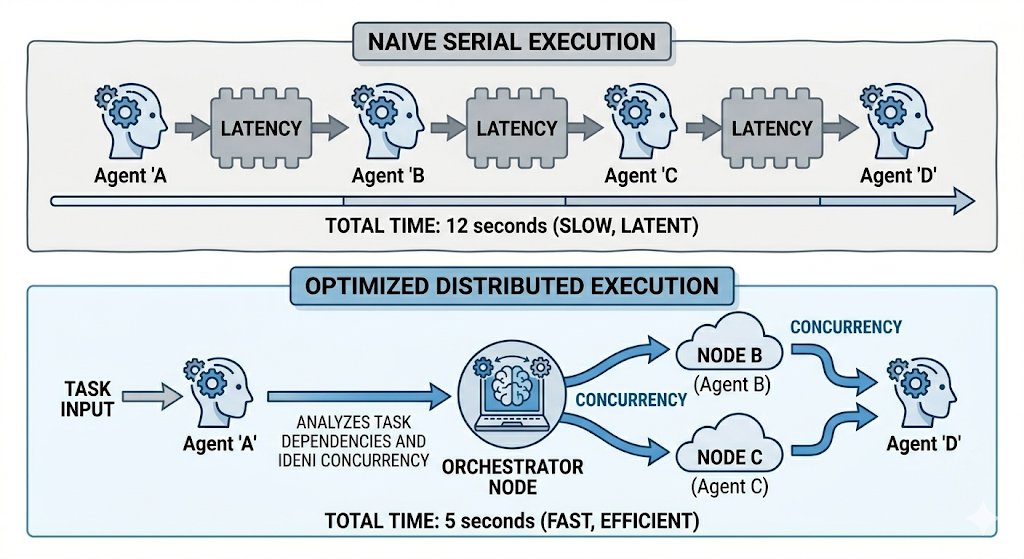
\includegraphics[width=\columnwidth]{figures/serial-vs-optimized.png}
\caption{Na\"ive serial execution (top) versus optimized distributed
  execution (bottom). The optimizer identifies independent task nodes
  and schedules them concurrently, reducing total latency from the sum
  of all node times to the critical path length.}
\label{fig:serial-vs-optimized}
\end{figure}

\noindent\textbf{Redundant node elimination.} If the user's original
prompt already contains the data that a proposed fetch node would
retrieve, the optimizer can eliminate the redundant node entirely,
analogous to dead code elimination in traditional compilers.

\noindent\textbf{Model tier selection.} Not every node requires the most
capable (and expensive) model. A simple data formatting step can be
handled by a fast, inexpensive model, while a complex reasoning step
warrants a more powerful one. The optimizer can assign model tiers based
on task complexity, reducing both cost and latency without sacrificing
output quality.

\subsection{Phase 4: Code Generation---Stateful Orchestration}
\label{sec:arch:codegen}

The final phase of a compiler generates executable machine code for the
target environment. The compiled binary manages CPU state, registers,
and memory. For multi-agent systems, the orchestrator \emph{is} the
target environment, and ``code generation'' means constructing a
stateful execution plan that manages the distributed system's lifecycle.

Figure~\ref{fig:orchestrator} shows the stateful orchestration control
loop. The orchestrator node---analogous to the compiled binary's runtime
---performs three functions:

\begin{figure}[t]
\centering
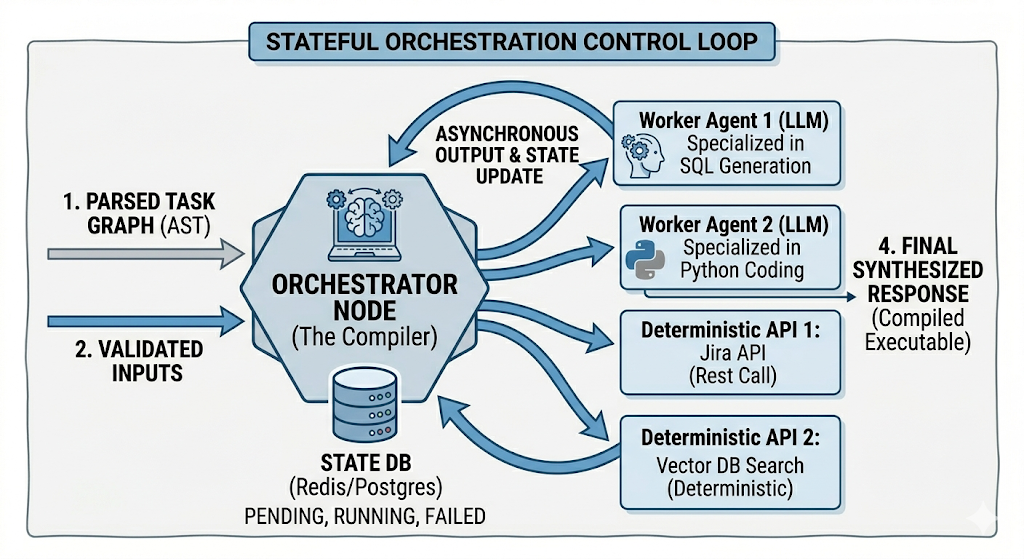
\includegraphics[width=\columnwidth]{figures/state-machine-based-orchestrator.png}
\caption{The stateful orchestration control loop. The orchestrator
  manages a parsed task graph, maintains execution state in a persistent
  store, dispatches work to heterogeneous worker agents and deterministic
  APIs, and synthesizes the final output.}
\label{fig:orchestrator}
\end{figure}

\noindent\textbf{Persistent state management.} Using a database (Redis,
Postgres, or an in-memory store), the orchestrator maintains the state
of the entire task graph: which nodes are pending, which are running,
which have completed, and which have failed. This state persistence
enables recovery from partial failures without re-executing the entire
pipeline.

\noindent\textbf{Heterogeneous dispatch.} The orchestrator coordinates
both LLM-based worker agents and traditional deterministic services. A
SQL query node dispatches to a database client, not an LLM. A vector
search node dispatches to an embedding index. Only tasks that genuinely
require language understanding are routed to LLM agents. This
heterogeneity is a key advantage over prompt-only architectures, which
route everything through expensive language models regardless of
whether the task requires one.

\noindent\textbf{Output synthesis.} The orchestrator aggregates the
results of distributed task nodes into a coherent final response,
respecting the dependency ordering established by the Abstract Task
Tree.

% ══════════════════════════════════════════════════════════════════════════════
\section{Implementation: A Self-Hosted Agentic Compiler}
\label{sec:implementation}
% ══════════════════════════════════════════════════════════════════════════════

To validate the architecture, we implement it as a self-hosted agentic
compiler written in Orca. The compiler takes natural language
descriptions of desired agent workflows and generates valid
\texttt{.orca} source files, which are then compiled by the Orca compiler
into executable Python/LangGraph code.

\subsection{The Two-Stage Pipeline}
\label{sec:impl:pipeline}

The implementation creates a two-stage compilation pipeline with a
critical property: \emph{non-determinism is isolated to the first
stage}.

\begin{enumerate}[leftmargin=*]
  \item \textbf{Stage 1 (non-deterministic):} Natural language
        $\xrightarrow{\text{agentic compiler}}$ \texttt{.orca} files.
        This stage uses LLM agents and is inherently non-deterministic.
  \item \textbf{Stage 2 (deterministic):} \texttt{.orca} files
        $\xrightarrow{\text{Orca compiler}}$ Python/LangGraph code.
        This stage is a traditional compiler---fully deterministic, with
        static type checking, reference resolution, and schema
        validation.
\end{enumerate}

The key insight is that Stage~2 acts as a \emph{safety net} for
Stage~1. If the LLM-based agentic compiler produces malformed output---a
type mismatch, an undefined agent reference, a missing required
field---the Orca compiler catches it at compile time with a precise
diagnostic, before any generated code reaches execution. This is
analogous to how a type checker catches bugs in hand-written code, but
here it catches bugs in \emph{machine-generated} code.

\subsection{Bootstrapping}
\label{sec:impl:bootstrapping}

The agentic compiler is itself written in Orca, demonstrating the
language's expressiveness for defining AI systems. This self-hosting
property---a compiler that compiles itself---has a long tradition in
programming language design (GCC, Rust, Go), and its presence here
serves as both a validation of Orca's expressive power and a practical
demonstration of the architecture.

The seed implementation defines the four pipeline phases as Orca agents:

\begin{lstlisting}[caption={Seed implementation of the agentic compiler
  in Orca (simplified). The prompt analyst decomposes natural language
  into structured steps.},label={fig:orca-compiler}]
model gpt {
  provider   = "openai"
  model_name = "gpt-4o"
}

agent prompt_analyst {
  model   = gpt
  persona = ```
    You are a prompt analyst. When the user
    gives you a prompt for a workflow, break
    it down into a list of steps. If the
    prompt is ambiguous, report the error
    instead of guessing.
    ```
  output = schema {
    @desc("The decomposed steps")
    steps = list[string] | null
    @desc("Error if prompt is ambiguous")
    error = string | null
  }
}

workflow compile {
  flow = prompt_analyst -> {
    "steps": code_generator,
    "error": error_reporter,
  } -> end
}
\end{lstlisting}

The \texttt{prompt\_analyst} agent acts as the parser (Phase~1),
producing structured output with a typed schema. The workflow's
conditional routing (\texttt{"steps"} vs.\ \texttt{"error"}) implements
the semantic validation (Phase~2): ambiguous input is rejected rather
than propagated.

\begin{todobox}
Expand the seed implementation to include all four phases as distinct
agents: validator, optimizer, and code generator. Show the complete
\texttt{orca.orca} once the full pipeline is implemented.
\end{todobox}

% ══════════════════════════════════════════════════════════════════════════════
\section{Discussion}
\label{sec:discussion}
% ══════════════════════════════════════════════════════════════════════════════

\subsection{Why This Matters for Systems Architects}
\label{sec:discussion:architects}

The compiled approach is fundamentally about engineering rigor. By
applying compiler design principles, we build multi-agent systems where
intelligence is centralized in the \emph{architecture}, not in the
prompts. This shift yields three properties that ad hoc prompt chains
lack:

\noindent\textbf{Observability.} When execution fails in a compiled
system, the developer does not debug a hallucination. They see exactly
which node in the task graph failed and why---a semantic validation
failure for a missing permission, a schema mismatch at an agent
interface, or a context window overflow. The Abstract Task Tree provides
the same structured traceability that a compiler's AST provides for
source-level debugging.

\noindent\textbf{Reliability.} With typed interfaces and schema
enforcement at every boundary, distributed agents become replaceable
microservices that produce structured outputs according to a shared
contract. An agent can be swapped, upgraded, or replaced with a
deterministic API without affecting the rest of the pipeline, just as a
compiler backend can be swapped without changing the frontend.

\noindent\textbf{Scalability.} When we stop chaining monolithic prompt
sequences and start compiling modular intent graphs, we unlock the
performance benefits of concurrent, distributed execution. Independent
task nodes execute in parallel; only the critical path determines
end-to-end latency.

\subsection{Limitations}
\label{sec:discussion:limitations}

\begin{todobox}
Discuss limitations:
\begin{itemize}
  \item The Parser Agent itself relies on an LLM, so the initial
        decomposition is still non-deterministic. Mitigations: structured
        output schemas, validation feedback loops.
  \item Complex workflows with deep conditional logic may resist clean
        decomposition into a static task graph.
  \item The optimization phase currently relies on heuristics rather
        than formal cost models for model tier selection.
\end{itemize}
\end{todobox}

% ══════════════════════════════════════════════════════════════════════════════
\section{Evaluation}
\label{sec:evaluation}
% ══════════════════════════════════════════════════════════════════════════════

\begin{todobox}
Evaluate the architecture:
\begin{itemize}
  \item \textbf{Correctness}: Test with N natural language prompts of
        varying complexity. Measure the percentage that produce valid
        Orca output and working agent systems.
  \item \textbf{Concurrency gains}: Compare serial vs.\ optimized
        execution times on task graphs with independent nodes.
  \item \textbf{Error detection}: Catalog errors caught by semantic
        validation that would have caused runtime failures in a prompt
        chain.
  \item \textbf{User study}: Compare time-to-working-system for
        natural language $\rightarrow$ Orca vs.\ hand-written Orca vs.\
        raw Python/LangGraph.
\end{itemize}
\end{todobox}

% ══════════════════════════════════════════════════════════════════════════════
\section{Related Work}
\label{sec:related}
% ══════════════════════════════════════════════════════════════════════════════

\noindent\textbf{Agent frameworks.}
LangGraph~\cite{langgraph} provides graph-based orchestration but
requires imperative Python for all configuration and offers no static
analysis. AutoGen~\cite{autogen} simplifies multi-agent conversation
but lacks structured task decomposition. CrewAI~\cite{crewai}
introduces role-based agents with YAML configuration, moving toward
declarative definitions but without a type system or compiler. All three
implement variants of prompt chaining; none apply compiler design
principles to the orchestration itself.

\noindent\textbf{AI programming DSLs.}
DSPy~\cite{dspy} compiles declarative language model calls into
self-improving pipelines, applying a ``compilation'' metaphor to prompt
optimization. LMQL~\cite{lmql} extends Python with a query syntax for
constrained LLM generation. Both target individual model interactions
rather than multi-agent orchestration. Our work is complementary: DSPy
modules could serve as optimized tool implementations within an
Orca-orchestrated system.

\noindent\textbf{Code generation from natural language.}
General-purpose code generation tools (GitHub Copilot, Claude, Codex)
produce arbitrary code from natural language descriptions. Our approach
differs in targeting a constrained DSL rather than general-purpose
Python, which bounds the output space and enables compiler-verified
correctness---a property that general code generation cannot guarantee.

\noindent\textbf{Infrastructure DSLs.}
HCL/Terraform~\cite{terraform} is the closest analogue to our approach:
a declarative block language that compiles to imperative API calls. Orca
adapts HCL's philosophy to the agent domain, and the agentic compiler
adds a natural language frontend to this stack, creating a three-tier
architecture: natural language $\rightarrow$ DSL $\rightarrow$
executable code.

% ══════════════════════════════════════════════════════════════════════════════
\section{Future Work}
\label{sec:future}
% ══════════════════════════════════════════════════════════════════════════════

Several extensions are planned:

\begin{itemize}[leftmargin=*]
  \item \textbf{Iterative refinement.} A conversational loop where
        users refine the generated Orca code through follow-up prompts,
        with the compiler providing type-checked feedback at each
        iteration.
  \item \textbf{Visual frontend.} Combining the agentic compiler with a
        node-and-edge graph editor: natural language generates the
        initial graph, and users refine it visually.
  \item \textbf{Learning from corrections.} When a user manually fixes
        generated \texttt{.orca} code, feeding corrections back to
        improve future generation accuracy.
  \item \textbf{Multi-framework targeting.} Since Orca's language
        design is backend-independent, the same natural language prompt
        could target different execution frameworks (LangGraph, AutoGen,
        direct API calls).
  \item \textbf{Formal cost models.} Replacing heuristic-based
        optimization with formal cost models for model tier selection,
        informed by empirical latency and accuracy measurements.
\end{itemize}

% ══════════════════════════════════════════════════════════════════════════════
\section{Conclusion}
\label{sec:conclusion}
% ══════════════════════════════════════════════════════════════════════════════

As multi-agent AI systems grow in complexity, the gap between developer
intent and reliable execution widens. The prompt chaining paradigm---
connecting LLMs with natural language in ad hoc sequences---cannot
bridge this gap; it lacks the structural guarantees that production
systems demand.

We have presented an architecture that applies compiler design
principles to multi-agent orchestration: parsing user intent into a
structured task graph, validating it against semantic constraints,
optimizing it for concurrency and cost, and generating a stateful
execution plan. Each phase provides the same benefits in the agent
domain that its compiler analogue provides for source code:
structured error reporting, type safety, optimization, and
deterministic output.

Our implementation as a self-hosted agentic compiler in Orca
demonstrates both the architecture's feasibility and a practical
two-stage pipeline that isolates LLM non-determinism from deterministic
compilation. The engineers who build the most robust multi-agent systems
will be those who treat LLMs not as autonomous agents to be chained
together, but as powerful, non-deterministic components that require the
same structural constraints that compilers impose on code. The path
forward is not smarter prompting---it is smarter engineering.

% ══════════════════════════════════════════════════════════════════════════════
% References
% ══════════════════════════════════════════════════════════════════════════════
\bibliographystyle{ACM-Reference-Format}
\bibliography{references}

\end{document}
